
\thispagestyle{empty}

\chapter{Integration of ocular and vestibular signals for self-motion perception in darkness}
\chaptermark{}

\label{p3}

\newpage

\small {\bf Abstract} Self-motion is typically accompanied by compensatory eye movements that help minimise retinal slip and maximise dynamic visual acuity. To date, it is unknown whether these eye movements also have a reversed role, serving as a cue for self-motion perception. To address this question, we had participants ($n=8$) judge self-motion during different eye movement conditions in the absence of full-field optic flow.  In a 2AFC task, participants indicated whether the second of two successive passive lateral whole-body translations was longer or shorter than the first. Eye movements during each translation were world-stationary, or body-stationary in an otherwise dark room. Results of these two conditions show that the perceived translations were shorter with body-fixed gaze compared to world-fixed gaze. Using a linear model, we estimated the relative contributions of vestibular and eye movement signals to self-motion perception and found that eye movement signals contribute approximately 25 percent. The model was independently validated by successfully predicting the effects of eye movements on self-motion in a third condition without any visual fixation, i.e. when the eyes were free to move. We conclude that eye movement signals influence self-motion perception, even in the absence of visual stimulation, and even when oculomotor and vestibular estimates are in conflict, e.g. during body-fixed gaze. We hypothesise that adverse consequences of this seemingly inflexible arrangement are minimal under natural conditions because eye movements and self-motion are highly correlated, and because eye movements are most often accompanied by veridical optic flow cues to self-motion.

\vfill

\noindent\underline{ \hspace{4cm} }

\noindent This chapter is being revised for publication \newline
\noindent {\bf Clemens, I.A.H.}, Selen, L.P.J., MacNeilage, P.R. and Medendorp, W.P. \citeyear{clemens2015a}. %Title. \emph{Journal}, volume(issue): from-to. \newline

\newpage

%%%%%%%%%%%%%%%%
% Introduction %
%%%%%%%%%%%%%%%%

\section{Introduction}

An accurate estimate of self-motion is important to guide interactions with the environment. During passive self-motion both vestibular and optic flow signals provide information about self-motion \cite{gibson1955, benson1986, harris2000, israel1989, angelaki2005, carriot2013, chen2010}. However, also compensatory eye movements that maintain fixation on world-fixed objects carry self-motion information. These eye movements are driven by retinal slip or vestibular signals. For example, the linear vestibulo-ocular reflex (LVOR) stabilises gaze during head translations, even in complete darkness \cite{paige1989,medendorp2002,angelaki2004}.  Many studies have shown that the brain uses oculomotor signals to extract the optic flow component related to self-motion \cite{warren1988, royden1992, freeman1998, lappe1999}, but to our knowledge a direct influence of eye movements on self-motion perception has not been investigated. Here we study whether these oculomotor signals are also used to estimate self-motion directly.

When gaze is world-stable during whole-body translation, the eye displacement correlates with translation size and is modulated by fixation depth \cite{schwarz1989, paige1998, mchenry2000, medendorp2002}. When properly scaled this eye movement signal could serve as a self-motion cue. In contrast, when fixation is body-fixed the eyes remain stationary in their orbits \cite{paige1998, ramat2005} making them no longer informative about self-motion. If, however, the brain assumes that eye movements are always made to maintain world-stable gaze, as in the LVOR, it would equate the absence of eye movements with the absence of self-motion. As a result, self-motion with body-fixed gaze should be underestimated compared to self-motion with world-fixed gaze, despite identical vestibular cues.

This hypothesis implies that oculomotor signals are always combined with vestibular signals to estimate self-motion, even in complete darkness.  In this case, the size of the unconstrained eye movements should resemble a VOR movement that is intermediate between body- and world-fixed fixation, and should parametrically relate to the perceived self-motion.

To test whether eye movements are used in self-motion perception, we employed a two-alternative forced choice (2AFC) paradigm in which participants were presented with two consecutive lateral translations. They had to indicate whether the second translation was longer or shorter than the first. Eye movements during each interval were either constrained using a  body or world stationary fixation point or not constrained at all (i.e. free). We show that identical translations were perceived shorter when gaze was body stationary compared to world stationary. Furthermore, using a linear model we predicted perceived displacement during the free gaze condition based on vestibular signals and unconstrained eye movements. We conclude that eye movements influence self-motion perception even in the absence of optic flow or other visual stimulation.


%%%%%%%%%%%
% Methods %
%%%%%%%%%%%

\section{Materials and methods}
\label{p3:sec:methods}

\subsection{Participants}

Eight naive participants (three male, five female), aged between 22 and 29 years, provided written informed consent to participate in the experiment. All participants were free of any known vestibular or neurological disorder and had normal or corrected-to-normal visual acuity. Participants never received any feedback about their performance.

\subsection{Experimental setup}

A motorised linear sled \cite<see>[for details]{clemens2012} was used to laterally translate participants following a minimum jerk profile \cite{flash1985} of fixed duration (1 \si{\second}) and amplitudes ranging from 1 to 27 \si{\centi\metre}. Participants were seated on the sled such that the inter-aural axis aligned with the motion axis. They were restrained using a five-point seat belt and a chin rest. In addition, the head was held in place using a sled-fixed mold which resembled head-phones and pressed down on the head surrounding the pinnae. Auditory cues were suppressed using white noise presented through in-ear headphones. Experiments were conducted in complete darkness except for visual fixation points, projected by a laser pointer on a black bar 50 \si{\centi\metre} in front of the participant at eye level. Laser pointers used to project body-fixed targets were attached to the sled. Those used to project world-fixed targets were mounted on the wall behind the sled.

Eye movements were recorded at 500\si{\hertz} using an EyeLink II system (SR Research, Kanata, Canada) whose cameras were mounted to the sled and therefore remained stable with respect to the head during the entire experiment. Because the head and body positions were fixed during the experiment, the orientation of the eyes within the head, as measured by the tracker, was equivalent to the orientation of the eyes in space. The eye tracking system was calibrated before each session using 11 evenly spaced calibration points ranging from -22 to \siang{22} degrees. We used linear regression to link EyeLink measurements to gaze angles.

\subsection{Paradigm}
We used a two-alternative forced choice (2AFC) task to measure perceived linear self-motion across three different eye fixation types: world-fixed, body-fixed, and unconstrained (free) fixation. We refer to these as world, body and free, respectively. A trial contained two sequential translation intervals of equal duration (1 \si{\second}) and in the same direction (either leftward or rightward). Different fixation types were presented in the two translation intervals. Participants were instructed to judge whether the translation during the second interval was longer or shorter compared to the first interval. They were additionally instructed to always look at the fixation point when it was visible; no instructions were given for when the fixation point was switched off (i.e. during free fixation).


\begin{figure}
    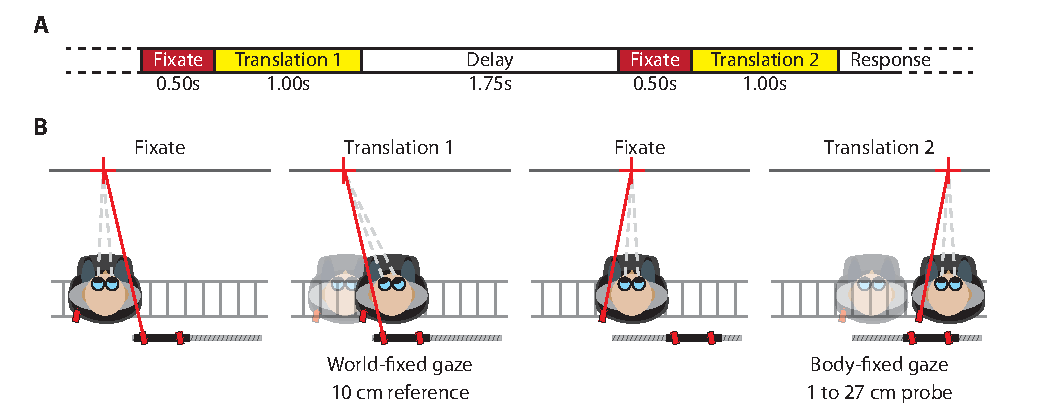
\includegraphics[width=1.0\textwidth]{src/paper3/figure1.pdf}

    \caption{\panel{A} Time course of key events within a single trial. In each of the two intervals, a 0.50 \si{\second} fixation period (red) precedes the lateral translation (yellow). A 1.75 \si{\second} long delay period (shown in white) separates the two intervals. After the second translation, the participant responded whether this second translation was longer or shorter than the first. \panel{B} Top-view illustrating key events during a body vs. world trial. First panel: participant fixates the world-fixed target (red cross) at the start of the first interval. Second panel: translation with world-fixed fixation target. Third panel: body-fixed fixation at start of second fixation interval. Fourth panel: translation with body-fixed fixation in second interval.}
    \label{p3:fig1}
\end{figure}

The time evolution of a single trial is shown in \figref{p3:fig1}. Each trial started with the onset of a central fixation point (i.e. aligned between the eyes) for 0.5 \si{\second}. Subsequently, the first translation interval commenced.  Depending on the fixation type, the fixation point remained visible (world and body) or was extinguished (free) during the translation interval. The trial shown in the figure depicts the 10 \si{\centi\metre} reference translation with world fixation. After this first interval, a delay followed in which the participant was kept in complete darkness for 1.75 \si{\second}. Then, the central fixation point reappeared, followed 0.5 \si{\second} later by the second interval, in which the probe translation was presented. The set of possible probe translations ranged from 1 to 27 \si{\centi\metre} in equidistant steps of 0.4 \si{\milli\metre}. The fixation type in the probe interval was always different than in the associated reference interval (the trial in \figref{p3:fig1} illustrates body fixation). After the second interval, the participant had to indicate whether he or she perceived the second translation as longer or shorter than the first using a 1-dimensional joystick. Moving the poke away from the body indicted that the second movement was longer, while moving it towards the body indicated that the second movement was shorter.


\begin{table}
    \begin{tabular}{llll}
    Comparison & Reference & 1st interval & Direction \\
    \hline
    Body vs. world & Body & Reference & Right \\
    & & & Left \\
    & & Probe & Right \\
    & & & Left \\
    \cline{2-4}
	& Body & Reference & Right \\
    & & & Left \\
    & & Probe & Right \\
    & & & Left \\
    \hline
    Body vs. free & Body & Reference & Right \\
    & & & Left \\
    & & Probe & Right \\
    & & & Left \\
    \cline{2-4}
	& Free & Reference & Right \\
    & & & Left \\
    & & Probe & Right \\
    & & & Left \\
    \hline
    World vs. free & World & Reference & Right \\
    & & & Left \\
    & & Probe & Right \\
    & & & Left \\
    \cline{2-4}
	& Free & Reference & Right \\
    & & & Left \\
    & & Probe & Right \\
    & & & Left \\
    \end{tabular}

    \caption{List of the three main comparisons that we tested. The (10 \si{\centi\metre}) reference movement was presented in either the first or second movement interval. We also manipulated movement direction (leftwards or rightwards), yielding a total of 24 trial types.}

    \label{p3:tab1}
\end{table}

Thus, a trial consists of two translations with different fixation types; in the three main conditions we compare the body versus world, world versus free, and body versus free fixation types. For each main condition, we varied which fixation type served as the reference stimulus and the order in which reference and probe were presented, which gives a total of four variations per main condition (see \tabref{p3:tab1}). In addition we varied translation direction (either leftward or rightward on consecutive trials). The amplitude of the probe translation was adaptively chosen using the Psi method. This method picks the amplitude for the next trial which maximises the expected decrease in entropy based on participants' responses to earlier trials \cite{kontsevich1999}. This was done separately for all 24 trial types (3 main conditions x 2 reference stimuli x 2 reference/probe orders x 2 translation directions; see \tabref{p3:tab1}). A total of 25 trials were collected per trial type yielding a total of 200 trials for each of the three main conditions.

Trials were presented in three one-hour sessions. To prevent dark adaptation, we turned on the lights for 5 \si{\second} after every block of 6 trials, and for at least 30 \si{\second} every 4 blocks. We made sure that each of the 24 unique trial types were presented once every 4 blocks. After each block, the adaptive procedure determined which translation amplitudes to test in the following block. To increase the number of data-points available to the adaptive psychometric procedure at the beginning of the experiment, we collapsed across translation direction and reference order for the first 10 trials of every condition. After those collapsed trials, the procedure ran separately for each of the 24 distinct trial types.

\subsection{Data analysis}

For each combination of the three main conditions, and  the two reference/probe orders (see \tabref{p3:tab1}), we quantified the perceived probe translation  by calculating the probability of the probe translation judged longer compared to the 10 \si{\centi\metre} reference translation as a function of actual probe translation, given by $x$. We used a maximum likelihood fit of a cumulative Gaussian function to summarise the psychometric data:

\begin{equation}
\label{p3:eq1}
P(x) = \lambda + (1 - 2\lambda) \frac{1}{\sigma \sqrt{2\pi}} \int_{-\infty}^{x}{e^{-(y-\mu)^2 / 2\sigma^2}}dy,
\end{equation}

in which $|x|$ represents the size of the absolute probe displacement. The mean of the Gaussian represents the point of subjective equality (PSE). The slope of the curve reflects the precision ($1/\sigma$) of reference-probe discrimination performance. Parameter $\lambda$, representing the lapse rate, accounts for stimulus-independent errors caused by subject lapses or mistakes and was restricted to small values ($\lambda < 0.06$. Fits were performed using the Psignifit toolbox \cite{wichmann2001,wichmann2001b}.

For each trial type (see \tabref{p3:tab1}), we also quantified eye movements, corrected for drift, based on initial fixation. The main source of drift were tiny lateral movements of the eye tracking cameras due to sled motion. We discarded trials containing blinks as well as trials in which the final eye position exceeded two standard deviations from the condition's average. Based on these criteria, 6.1\%, 3.6\% and 1.6\% of all trials were rejected based on errors in body, world, and free fixation respectively. In addition we rejected 1.2\% of all trials because participants blinked within the movement interval.

For the remaining trials, we computed the average ratio between the measured eye excursion, $\varphi_i$, and the angle that would be needed were the trial testing the world-fixed condition. The latter is computed by taking the arc-tangent of the actual translation distance, $m_i$, divided by the fixation depth, $d_i$, which for small $\varphi$ can be approximated by $g = \varphi m/d$. We computed this ratio, $g$, for every fixation type and interval (see \tabref{p3:tab1}). Ideally, for body-fixed trials $g = 0$, and for world-fixed trials $g = 1$. Using this ratio, we are able to compute the expected eye excursion, $\hat{\varphi} = gd/m$, for any given translation distance even those we did not explicitly measure.

\subsubsection{Model}
\label{p3:sec:model}

Using a simple cue integration model, we investigated whether inter-subject and inter-condition differences in the observed PSEs in conditions containing a translation under free fixation depend on actual eye movement behaviour. We modelled perceived distance, $p$, as a weighted linear combination of a vestibular and an oculomotor estimate of translation (\eqnref{p3:eq2}). We assumed that the vestibular estimate is equal to the actual translation, $m$, and that the oculomotor estimate is equal to expected eye movement given the  actual, $\hat{\varphi}_{m_i}$. As the weights represent the relative contributions of the oculomotor and vestibular systems, they can sum to any arbitrary value; in \eqnref{p3:eq2} their sum is fixed to 1. Thus, the weighting parameter $\alpha$ regulates the eye movement contribution and $1 - \alpha$  the vestibular contribution:

\begin{equation}
\label{p3:eq2}
p = \alpha \hat{\varphi}_m d + (1 - \alpha) m = \alpha g m + (1 - \alpha) m
\end{equation}

By definition, the probe displacement is perceived as equal in length to the 10 \si{\centi\metre} reference displacement at the PSE. By substituting both sides by the right hand side of \eqnref{p3:eq3} and using subscripts for reference ($r$) and probe intervals ($p$), we obtain:

\begin{equation}
\label{p3:eq3}
\alpha g_r m_r + (1 - \alpha) m_r = \alpha  g_p m_p \alpha + (1 - \alpha) m_p + \epsilon
\end{equation}

In the present experiment, the reference displacement, $m_r$, was always 10 \si{\centi\metre} and the probe displacement, $m_p$, was equal to the measured PSE for the presented combination of fixation types (i.e, $PSE$ in \eqnref{p3:eq1}). This model (i.e. \eqnref{p3:eq3}) was then fit to data from the body and world conditions using linear regression, finding weight α that minimises the sum of squared errors ($\sum{\epsilon^2}$).

\begin{equation}
\label{p3:eq4}
m_r - m_p = \alpha(g_{f_p} m_p - g_{f_r} m_r + m_r - m_p) + \epsilon
\end{equation}

By only using data from conditions where a visual fixation point was present during both translations (i.e. body versus world) to fit the model, we could examine whether the same weight $\alpha$ can also explain the PSEs found in the conditions containing a free fixation interval. To this end, we solved Equation 3 for $m_p$ and computed PSE estimates, $P\hat{S}E$, for the body versus free and world versus free conditions (\eqnref{p3:eq5}).

\begin{equation}
\label{p3:eq5}
\hat{m}_p = P\hat{S}E = \frac
	{\alpha g_r + (1 - \alpha)}
	{\alpha g_p + (1 - \alpha)}
    m_r
\end{equation}

In addition to minimizing the sum of squared errors in \eqnref{p3:eq4}, we also fit \eqnref{p3:eq5} to the data in order to see if weight $\alpha$ depends on the way the model is formulated. Parameters obtained by fitting \eqnref{p3:eq5} fell well within the standard deviation reported in \tabref{p3:tab2} for all participants, suggesting that they did not depend on the way the model was formulated.


%%%%%%%%%%%
% Results %
%%%%%%%%%%%

\section{Results}

The current experiments investigate the influence of fixation type and associated eye movements on the perception of self-motion. Participants were presented with two subsequent lateral translations (\figref{p3:fig1}) and they had to judge whether the second was longer or shorter than the first. During each interval participants fixated a body- or world-fixed target (body and world fixation) or were moved in absence of a fixation point (free fixation).

\begin{figure}
    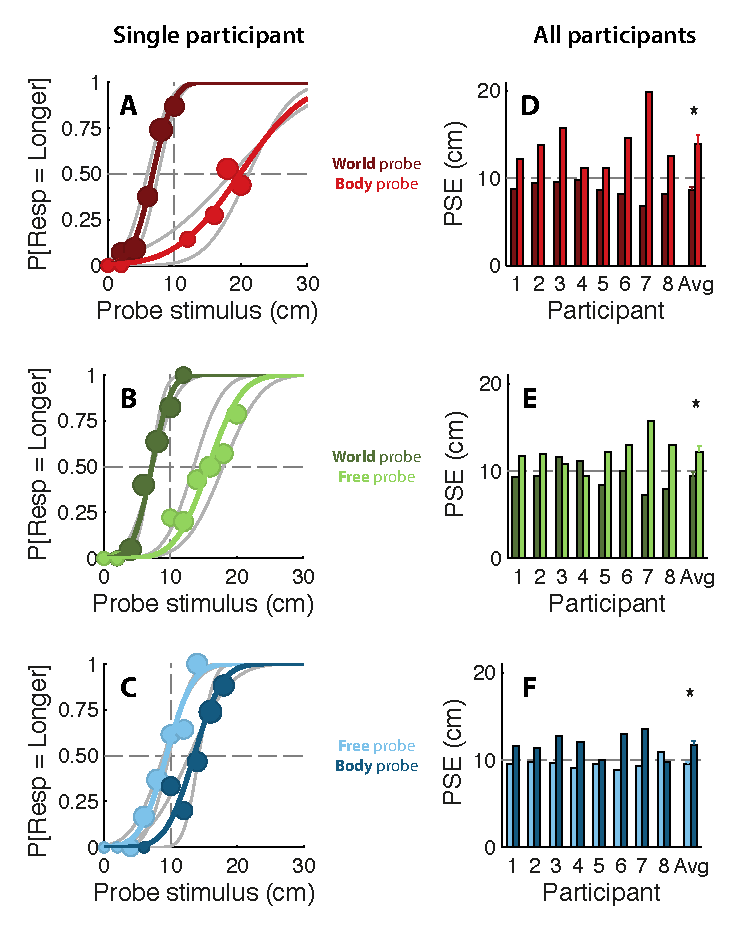
\includegraphics[width=1.0\textwidth]{src/paper3/figure2.pdf}

    \caption{Psychometric curves (coloured lines) and associated binned data (circles) for one participant (top row). Circle size represents the number of trials within each 2 \si{\centi\metre} bin. Binning was only done in order to visualise this participant's responses and was not used otherwise. Gray lines show psychometric curves before collapsing across reference order. \panel{A} Body-world comparison; body reference, dark red; world reference, light red. \panel{B} World-free comparison; world reference, light green; free reference, dark green. \panel{C}  Body-free comparison; body reference, dark blue; free reference, light blue. \newline
PSEs for all participants and the average {\textpm}SE (bottom row). \panel{D} Body-world (dark red) and world-body (light red) conditions. \panel{E} World-free (light green) and free-world (dark green) conditions. \panel{F} Body-free (dark blue) and free-body (light blue) conditions. Because a t-test revealed a main effect of reference order, \ttest{47}{-5.2}{0.01}, we used the mean PSE across reference order (e.g. \figref{p3:fig3}, gray lines) instead of the PSE collapsing across reference order (e.g. \figref{p3:fig3}, coloured lines); these values were not significantly different.}
    \label{p3:fig2}
\end{figure}

The performance of one participant is illustrated in the left column of \figref{p3:fig2}. Each row shows one main condition: body versus world fixation (top/red), world versus free fixation (middle/green), and body versus free fixation (bottom/blue). The lighter and darker colours in each panel indicate which fixation type was the reference movement (see Legend). The shift of the psychometric functions relative to the 10 \si{\centi\metre} reference (i.e. the PSE) quantifies the influence of fixation type. For example, the rightward shift of the light red curve in \panelref{p3:fig2}{A} means that for a body fixation a longer translation (\about 19 \si{\centi\metre}) was required for that translation to be perceived equivalent to a 10\si{\centi\metre} reference translation with world fixation. On the other hand, the leftward shift of the dark red curve means that a shorter translation with world fixation (\about 7 \si{\centi\metre}) was required for that translation to be perceived equivalent to the 10 \si{\centi\metre} reference translation with body fixation. Together, these oppositely directed shifts demonstrate that translations with world fixation were perceived longer than equivalent translations with body fixation, regardless of which translation was the reference.  Similarly, the shifts in \panelref{p3:fig2}{B} shows that world fixation translations were also perceived to be longer than free fixation movements and \panelref{p3:fig2}{C} shows that free fixation translations were perceived to be longer than body fixation translations. Note that \figref{p3:fig2} also shows effects on slope, which will be further discussed in the paragraph \nameref{p3:sec:precision}.

Similar results were obtained for all subjects, as shown by the individual PSEs for all participants (right column of \figref{p3:fig2}). Statistical significance of the fixation-induced effects for each main condition (world versus body, \panelref{p3:fig2}{D}; world versus free, \panelref{p3:fig2}{E}; and free versus body, \panelref{p3:fig2}{F}) was evaluated by comparing PSEs between the two reference conditions using a paired t-test. These PSEs were significantly different in all cases (world versus body, \ttest{7}{-4.09}{0.05}; world versus free, \ttest{7}{-2.48}{0.05}; free versus body, \ttest{7}{-3.38}{0.05}. As for the example subject, these results indicate that translations made with body fixation are perceived shorter than with world fixation, suggesting that self-motion perception is modulated by eye movements even in absence of full-field optic flow. The free fixation translations, which control for confounds of the small fixation point, were perceived to be longer than body and shorter than world fixation translation intervals, which could be expected if their gains were smaller than 1 but larger than 0.

\begin{figure}
    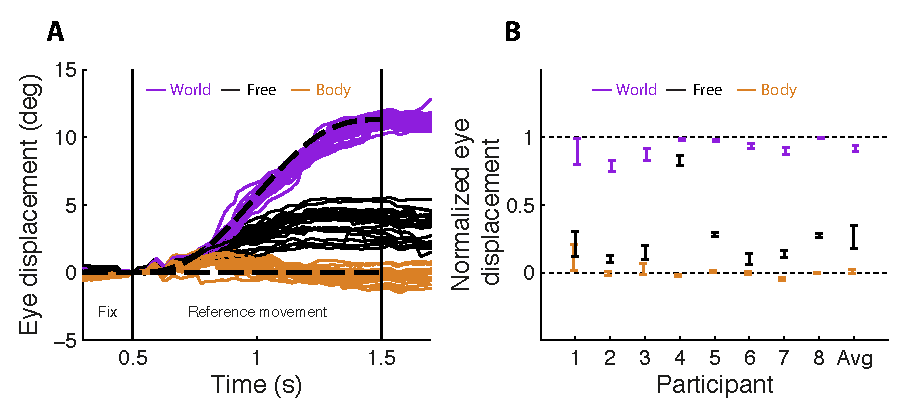
\includegraphics[width=1.0\textwidth]{src/paper3/figure3.pdf}

    \caption{\panel{A} Actual (solid lines) and ideal (dashed lines) eye movement traces of one participant during world fixation (purple), body fixation (brown), and free fixation (black). All traces shown are for 10 \si{\centi\metre} reference movements. \panel{B} Normalised eye position for each participant (\textpm95\% confidence interval) at the end of translation interval (error bars) for world fixation (purple), body fixation (brown) and free fixation (blue). In addition, the average {\textpm}SE across all participants is shown. Zero indicates that the eyes remained stationary relative to the body, and one indicates that eye position was perfectly world-fixed.}
    \label{p3:fig3}
\end{figure}

\subsection{Eye movement contributions to self-motion perception}

In order to relate psychophysical performance to eye movement behaviour we recorded and analysed eye movements during both intervals of every trial for all subjects. Exemplar eye traces for the 10 \si{\centi\metre} reference translation for the three fixation types are depicted in \panelref{p3:fig3}{A}. Fixation behaviour was quite accurate for both body fixations, where no eye movements were expected, and world fixation, where eye movement excursions of \siang{11} were expected, seemingly supported by  catch-up saccades. Under free fixation, the amount of eye movement was intermediate between body and world fixation and behaviour was more variable. A similar pattern was observed in all participants, as illustrated by the normalised eye movement data (see \nameref{p3:sec:methods}, and \panelref{p3:fig3}{B}).

\begin{figure}
    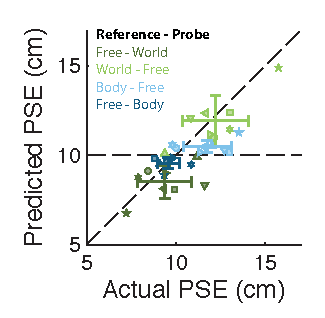
\includegraphics[width=0.5\textwidth]{src/paper3/figure4.pdf}

    \caption{Eye movement based prediction for the PSE plotted against the actual PSE.  A data point (symbol) is shown for each participant (symbol shape) and condition (symbol colour) pair, following the same colour scheme as in \figref{p3:fig2}. The identity line, corresponding to a perfect prediction, is shown in black.}
    \label{p3:fig4}
\end{figure}

\begin{table}
    \begin{tabular}{llll}
    Participant & Parameter ($\alpha$) \textpm SD \\
    \hline
    1 & 0.27 (\textpm 0.04) \\
    2 & 0.27 (\textpm 0.05) \\
    3 & 0.35 (\textpm 0.04) \\
    4 & 0.06 (\textpm 0.04) \\
    5 & 0.13 (\textpm 0.03) \\
    6 & 0.33 (\textpm 0.04) \\
    7 & 0.58 (\textpm 0.02) \\
    8 & 0.21 (\textpm 0.02) \\
    \end{tabular}

    \caption{Estimated eye movement contribution ($\alpha$) to the perception of self-motion (see \eqnref{p3:eq5}). Standard deviations are based on a bootstrap for each participant.}

    \label{p3:tab2}
\end{table}

To quantify the role of eye movements in self-motion perception, we tested a linear model (see \nameref{p3:sec:model}) in which perceived translation is a weighted average of a vestibular estimate (equal to the actual translation) and an oculomotor estimate (equal to the normalised eye movement times the actual translation; \eqnref{p3:eq2}). This model contains a single free parameter ($\alpha$), which corresponds to the relative weight given to the oculomotor estimate. We fit this model to the two body versus world conditions and obtained the value of the oculomotor weight for every subject (\tabref{p3:tab2}). The average oculomotor weight is 0.25 \textpm0.12 (SD), indicating that the contribution of the eye movement signal to the self-motion estimate is about 25 percent. Note that participant 4, whose oculomotor weight is furthest from this mean ($\alpha = 0.06$), also shows a radically different eye movement gain during the free-fixation (see \panelref{p3:fig3}{B}). We then used these oculomotor weights along with the normalised eye movement values to predict the PSEs in the remaining four conditions according to \eqnref{p3:eq5}. The predicted PSEs are plotted against the actually observed PSEs in \figref{p3:fig4}. The positive correlation ($\rho = 0.78$, $p < 0.01$) between observed and predicted PSEs suggests that eye movements are indeed used in self-motion perception, even in the absence of a fixation point (i.e. during free fixation). Furthermore, the fact that data points generally cluster near the unity line shows that our simple model does reasonably well in predicting perceptual performance across subjects and conditions based on oculomotor weight and normalised eye movement magnitude only. This holds true even for subject 7 whose oculomotor weight (\tabref{p3:tab2}) was approximately double the average, yet whose data points remain close to the unity line.

\begin{figure}
    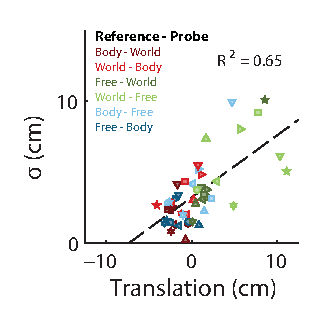
\includegraphics[width=0.5\textwidth]{src/paper3/figure5.pdf}

    \caption{Effect of difference movement amplitude between reference and probe interval (i.e. the bias) on response uncertainty ($\sigma$). A data point is shown for every participant and condition (symbol colour) pair, following the same colour scheme as in \figref{p3:fig2}. The dashed black line is the linear regression trend line.}

    \label{p3:fig5}
\end{figure}

\subsection{Precision depends on PSE}
\label{p3:sec:precision}

The psychometric curves of the example participant in \figref{p3:fig2} show that precision ($\sigma^{-2}$ in \eqnref{p3:eq1}) decreases as the difference between the PSE and the reference (i.e. the bias) increases. In \figref{p3:fig5} precision is plotted as a functions of bias for all participants and all conditions, showing a significant linear relationship ($R^2 = 0.64$) between the two. This effect, which follows Weber's perceptual law \cite{fechner1860} is consistent with the signal-dependence of (discrimination) precision that has been shown recently for vertical self-motion \cite{nesti2014}.


%%%%%%%%%%%%%%
% Discussion %
%%%%%%%%%%%%%%

\section{Discussion}

We investigated the contribution of eye movements to the perception of passively-induced self-motion. Experiments were performed in the absence of full-field optic flow to eliminate the contribution of this visual motion signal. Perception of self-motion was compared across three fixation types: during free fixation the fixation target was extinguished before the movement, while during world and body fixation, targets  remained stable relative to the world and body, respectively. Our results show that self-motion is underestimated during body fixation (in which the eyes remain stationary) compared to world fixation (in which the eyes move to maintain fixation).The eye movements during free fixation, which  are driven by the VOR, show a non-unity gain with excursions in-between body- and world-fixation conditions. Self-motion perception reflects this pattern of eye movements, suggesting an important contribution of this extraretinal signal to the perception of self-motion.

 To quantitatively characterise the separate vestibular and eye movement contributions, we fit a single parameter model to the perceptual responses for the body versus world comparison conditions and validated this model independently by predicting the effects of eye movements on self-motion perception during free fixation conditions. This model takes into account subject specific oculomotor weight and eye movement patterns. Based on these inputs it accurately predicts the responses in the free fixation conditions. This demonstrates that extra-retinal eye movement signals are used as a cue in the perception of self-motion, contributing significantly to the self-motion percept with a weight of approximately 25 percent, even in the absence of optic flow.

It is surprising that an influence of eye movements can be observed even for body- stationary fixations, during which the stationary eye movement signal is clearly in conflict with the non-zero vestibular signal. While this demonstrates the strength of the assumption that fixation targets are world-stationary, it raises the question how reliable this assumption is. Simultaneous recording of angular head and eye movements during natural behaviour reveals that approximately 80 percent of eye movements can be classified as compensatory, i.e. eye movements directed opposite to head movement and therefore consistent with maintenance of world-fixed fixation \cite{einhauser2007}. Similarly, other studies have shown that world-stationary fixations are common for many every day activities, ranging from making a cup of tea \cite{hayhoe2014} to driving a car \cite{land1994}, to walking \cite{foulsham2011} and even reaching, where people tend to look at the source and destination of the object, but not at the hand \cite{flanagan2003}. Because world-stationary fixations are so common, the natural world statistics imply that self-motion and eye movements are highly correlated, thus making eye movements a fairly reliable cue for self-motion.

Even when fixation is not world-fixed, eye movement signals are combined with optic flow signals to yield realistic self-motion estimates \cite<e.g>{royden1992, vandenberg2000}. During world-fixed fixation, the eyes move to compensate for body translation, thereby reducing the optic flow component in the retinal signal. The self-motion estimate will therefore be driven predominantly by the eye movement signal. On the other hand, in the body-fixed condition, eye movements are minimal and optic flow maximal such that perceived self-motion will be driven predominantly by the optic flow signal itself. Because our experiment was performed in darkness, this optic flow signal was absent in the body-fixed condition which can explain why self-motion was underestimated.

During body and world fixation, eye movements are driven by retinal slip of the fixation target. However, in the free fixation condition, retinal slip is not available and resulting eye movements resemble the linear vestibulo-ocular reflex (LVOR), in that the gain relative to world fixation was \about0.4 (see \panelref{p3:fig3}{B}; \citeNP{ramat2003}). This reflex is thought to be driven by a double integration of the vestibular signal, converting the head acceleration signal from the otoliths to eye position \cite{green2007,walker2010}. If eye movements during free fixation are in fact vestibularly driven, then combination of this eye movement signal with the vestibular signal itself seems redundant. However such combination could reflect a strategy to reduce noise. Both the direct (vestibular) and indirect (LVOR) signals depend on integration of the linear acceleration signal and may be corrupted by independent noise sources. Combining them in a statistically optimal fashion will decrease the noise level towards the noise level of the original source signal \cite{faisal2008,clemens2011,fetsch2013}. The consequence of this integration will be a reduced self-motion estimate when the gain of the LVOR is less than 1, as we observed in the free condition.

\subsection{Alternative interpretations}

In the above, we suggest that eye movements themselves drive perception of self-motion. However, it is conceivable that a common correlate of eye movements, such as attention or visual motion influenced our results. In 1963, Guedry and Harris reported a substantial underestimation of displacement when their observers watched a small body-fixed target compared to displacements in the dark. They attributed their findings to an attentional shift from judgements of body displacement in the dark to judgements of target displacement in the fixation condition. We favor an explanation based on eye movement characteristics.  In their study, it is likely that the VOR caused eye movements  to occur during the translations in darkness. If these movements were used to augment self-motion perception, then the perception of such translations would be overestimated compared to translations made without eye movements, e.g. when fixating a body-fixed target. Because Guedry and Harris \citeyear{guedry1963} did neither record nor explicitly manipulate eye movements, they were not able to unveil their explicit role. Conversely, we did not manipulate attentional processes \cite{kitazaki2003}, so we cannot completely exclude the possibility they play a role.

Others have reported errors in the disambiguation of self and object-motion. Examples include the perceived motion of body-fixed visual targets during angular acceleration (the oculogyral illusion; \citeNP{carriot2011}), the apparent displacement of body-fixed stimuli during linear acceleration (the oculogravic illusion; \citeNP{graybiel1952}) and the apparent movement of world-stationary targets during self-motion in darkness \cite{dyde2008}. Similar disambiguation errors could cause the effects we observed. More specifically, if movement of the fixation point relative to the observer were always attributed to self-motion, then self-motion would be underestimated during body relative to world fixation, as we observed. However, such attribution errors cannot account for the effects in the free condition, because no fixation point was visible and no attribution was required. In the free condition, we demonstrate that eye movements by themselves, occurring in the absence of visual tracking and other external cues, influence the perception of self-motion.

\subsection{Implications for other studies}

Many previous self-motion studies have used a body-fixed fixation point to control for eye movement related effects. Our results suggest, however, that using a body-fixed fixation point causes underestimation of self-motion. For example, Li, Wei, and Angelaki \citeyear{li2005a} investigated spatial updating across lateral translation and found that saccades to updated targets undershot the actual target location. As self-motion perception drives this update, the effects of eye movements on self-motion perception should also influence the updating process. In other words, the observed undershoot could be due to the underestimation of self-motion caused by the body-fixed fixation point. Another example is a study on the perception of vertical object-motion during lateral translation \cite{dokka2013}. This study reports incomplete compensation for self-motion when judging the deviation from vertical motion of a moving object. This observation could also be due to underestimation of self-motion induced by the fixation of the body-fixed target.

A moving fixation point is also known to influence self-motion perception, as in the Slalom Illusion \cite{freeman2000}; observers viewing expanding optic flow while fixating a target that oscillates from left to right perceive slaloming motion which is inconsistent with the purely forward motion specified by the expanding optic flow display. However, this observation is consistent with the idea that oculomotor signals are used in estimating self-motion. Additionally, it has been shown that eye movements affect postural sway \cite{glasauer2005}.  Participants performed smooth pursuit eye movements in complete darkness and displayed lateral sway consistent with the stabilization of posture using a self-motion estimate influenced by pursuit eye movements.

Studies conducted to characterise vestibular-only sensitivity are often performed in complete darkness or with closed eyes \cite{grabherr2008,  macneilage2010b, macneilage2010a, roditi2012, valko2012, nesti2014}. However, the results of our free-fixation condition suggest that even under these circumstances, results could easily be influenced by vestibularly driven eye movements. Overall, we suggest that any study concerned with self-motion processing must consider the possible influence of eye movements.

\subsection{Possible neural substrate}

This leaves us with the question of where in the brain these effects originate. The locus of our effect is likely to carry both eye movement and vestibular signals. Prime candidate areas known to carry both vestibular and eye movement signals are the vestibular nuclei \cite{henn1974,daunton1979} and the cerebellum \cite{waespe1981}. On the other hand, eye movements could influence self-motion perception indirectly via optic flow processing. In particular, cortical areas that carry both vestibular and optic flow signals (which can be modulated by eye movements) include the ventral intraparietal area (VIP; \citeNP{bremmer2002,chen2011}), and the dorsal medial superior temporal area (MSTd; \citeNP{gu2008}). Future work should reveal how such brain areas, directly or indirectly, merge both vestibular and oculomotor signals into a coherent percept of self-motion.
